\section{Istruzioni d'uso -- Operatore}

L'interfaccia Operatore \`e accessibile esclusivamente agli utenti con ruolo \texttt{admin}. Al login, se le credenziali appartengono a un operatore, viene effettuato un redirect automatico da \texttt{/} a \texttt{/operatore}.

L'interfaccia presenta un layout desktop con barra di navigazione laterale contenente tre sezioni: \textbf{Ticket Aperti}, \textbf{Storico Ordini}, \textbf{Profilo}. In alto a sinistra \`e visibile il nome dell'operatore; in alto a destra il pulsante di logout.

All'accesso, se \`e configurata una cartella di export, viene eseguito automaticamente un export batch degli ultimi ordini (fino a 50) e viene mostrata una notifica toast con il risultato.

\subsection{Dashboard e gestione ticket}

\begin{figure}[H]
    \centering
    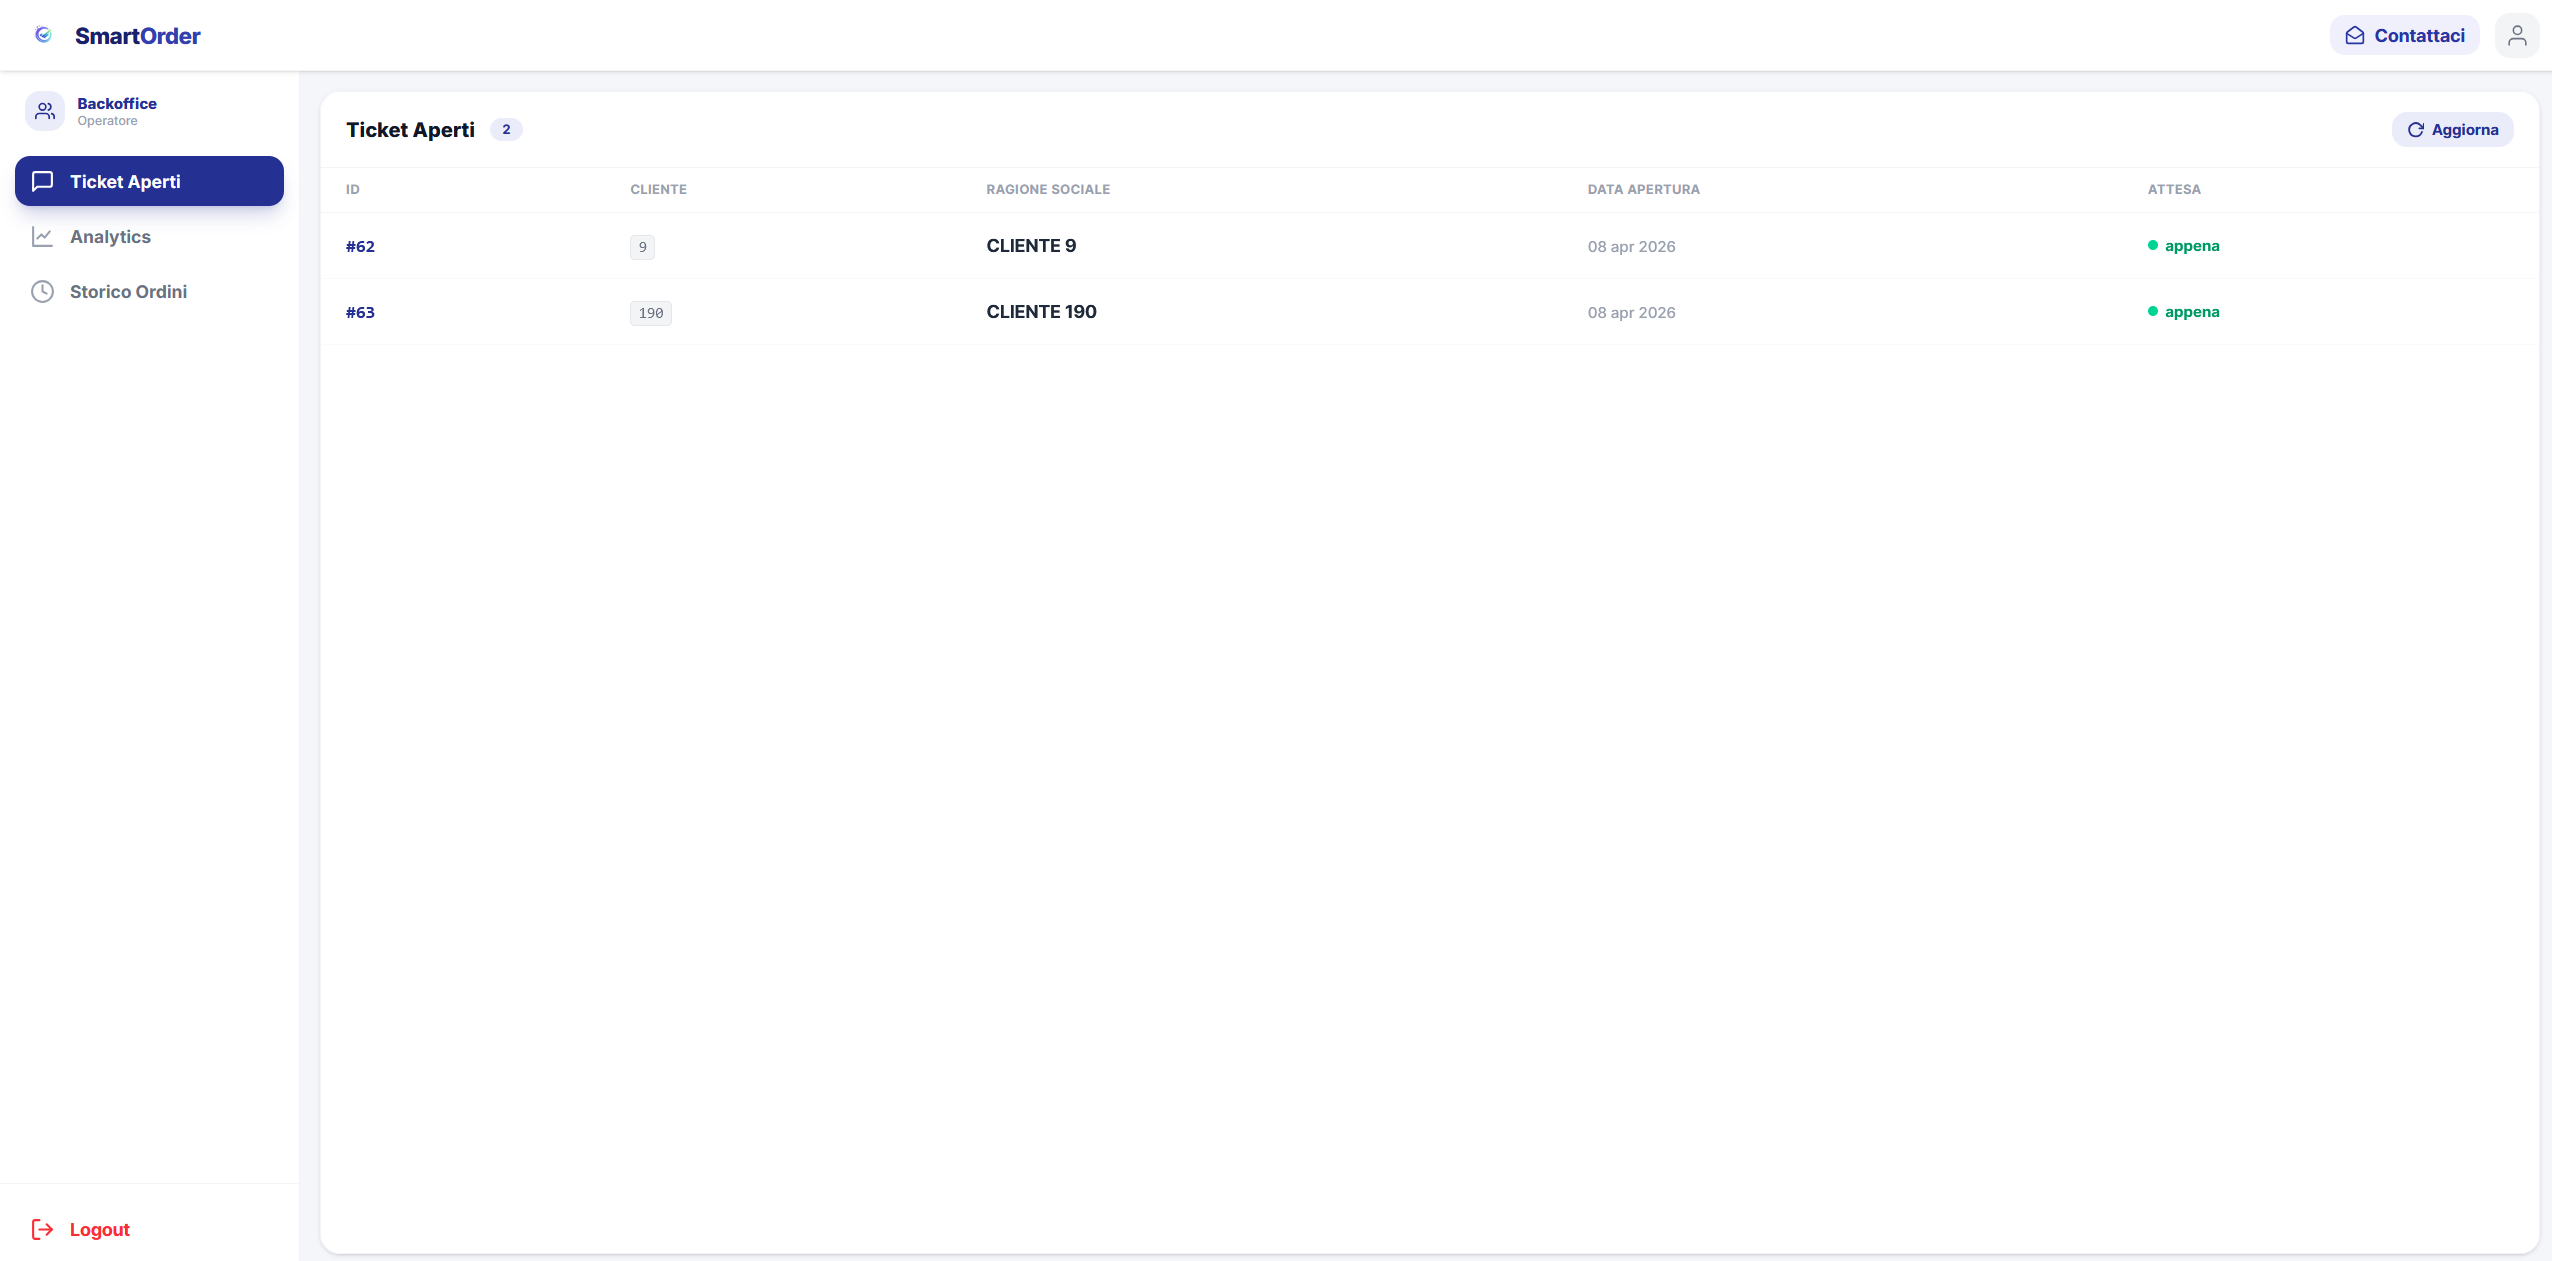
\includegraphics[width=0.7\textwidth]{Contenuti/immagini/lista ticket.png}
    \caption{Lista ticket aperti}
\end{figure}

La sezione \textbf{Ticket Aperti} \`e la vista predefinita dell'interfaccia operatore.

\subsubsection{Lista ticket}
\begin{enumerate}
    \item \textbf{Visualizzazione}: La tabella mostra tutti i ticket aperti e in lavorazione, ordinati per tempo di attesa decrescente (i pi\`u urgenti in cima). Ogni riga contiene: ID ticket, codice cliente (badge), ragione sociale, data di apertura e tempo di attesa.
    \item \textbf{Indicatore di gravit\`a}: Il tempo di attesa \`e colorato: rosso pulsante ($> 30$ minuti, urgente), ambra ($10$--$30$ minuti), verde ($< 10$ minuti).
    \item \textbf{Stato ticket}: Se un ticket \`e \texttt{In carico} (un operatore lo sta gi\`a gestendo), compare un badge ambra sulla riga.
    \item \textbf{Aggiorna}: Cliccare su \texttt{Aggiorna} in alto a destra per ricaricare la lista. L'elenco si aggiorna automaticamente anche in tempo reale tramite SSE.
    \item \textbf{Apertura ticket}: Cliccare su una riga qualsiasi per aprire il pannello di gestione del ticket.
\end{enumerate}

\subsubsection{Pannello di gestione ticket}

\begin{figure}[H]
    \centering
    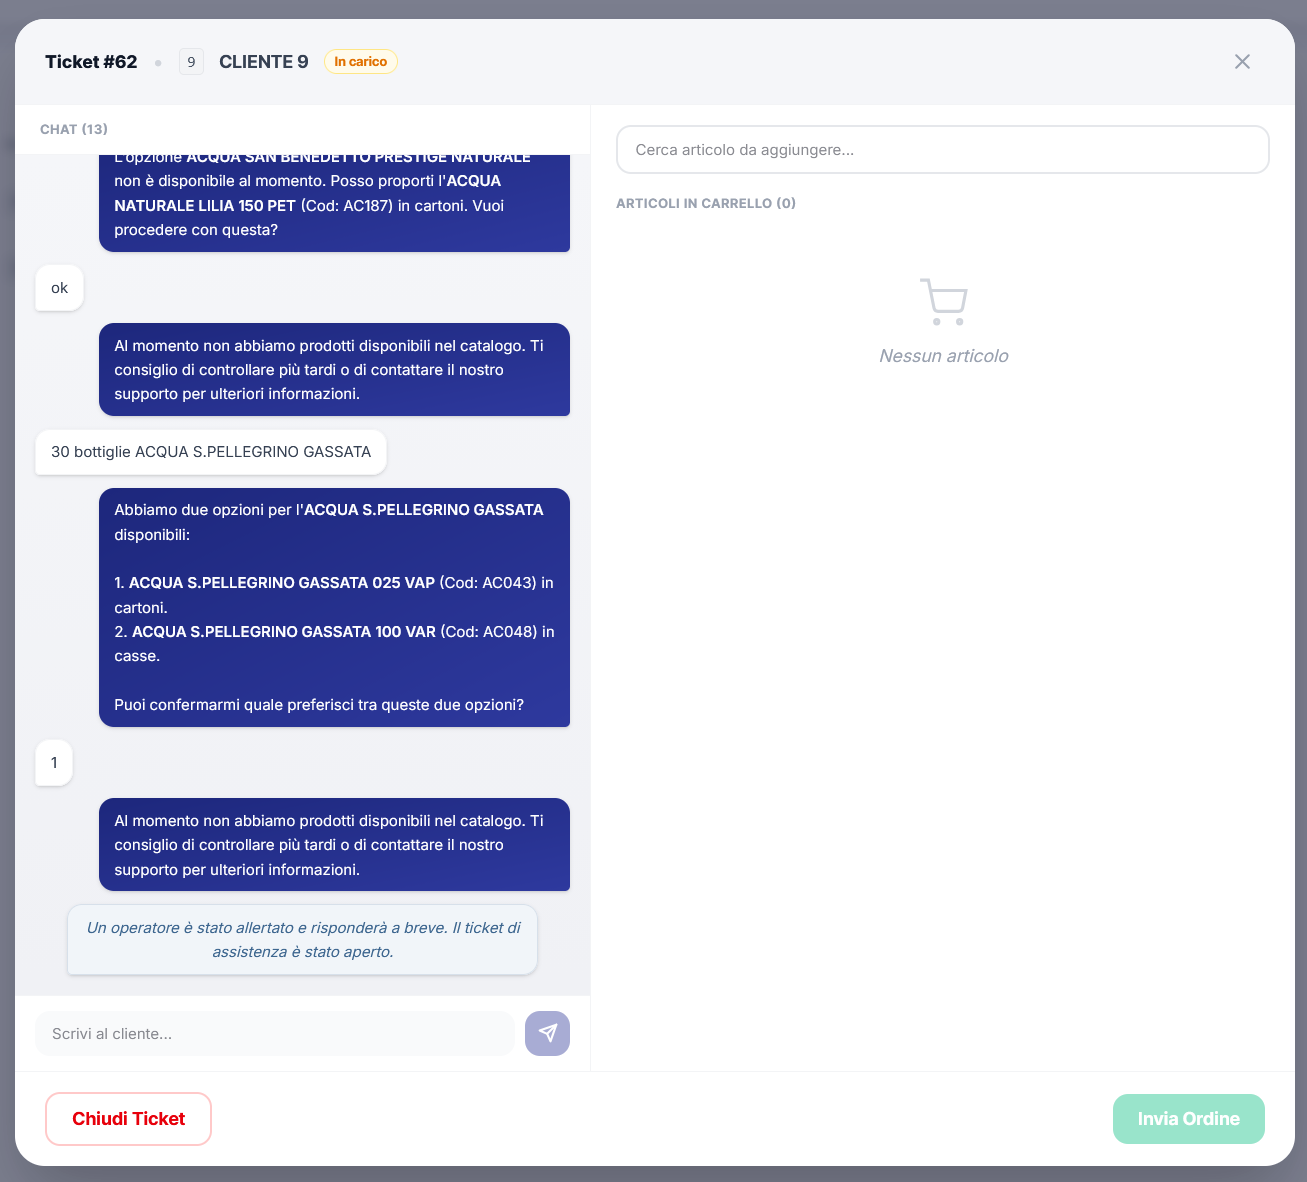
\includegraphics[width=0.7\textwidth]{Contenuti/immagini/ticket.png}
    \caption{Finestra di gestione ticket}
\end{figure}

Aprendo un ticket si accede a un modale a schermo intero suddiviso in tre aree:

\textbf{Header}: mostra l'ID ticket, il codice cliente, la ragione sociale e un badge di stato (Aperto o In carico). \`E presente il pulsante di chiusura (X).

\textbf{Area centrale sinistra (45\%)} -- \textbf{Chat}:
\begin{itemize}
    \item Elenco dei messaggi scambiati con il cliente (sia via IA che direttamente con l'operatore).
    \item I messaggi di sistema sono visualizzati in grigio corsivo centrato (ad esempio per segnalare che il ticket \`e stato aperto/assegnato).
    \item Vengono segnati i feedback inviati dai clienti
    \item Campo di input in basso per inviare messaggi di testo al cliente.
    \item I nuovi messaggi arrivano in tempo reale tramite SSE.
\end{itemize}

\textbf{Area centrale destra (55\%)} -- \textbf{Carrello Cliente}:
\begin{itemize}
    \item Campo di ricerca prodotti con autocomplete per aggiungere articoli al carrello del cliente.
    \item Elenco degli articoli attualmente nel carrello con possibilit\`a di modificarne le quantit\`a (pulsanti \texttt{+} e \texttt{-}) e rimuoverli (icona cestino).
    \item Badge \texttt{AI} e anello di confidenza per articoli aggiunti dall'IA.
    \item Il carrello si sincronizza in tempo reale sia con le azioni dell'operatore che con quelle del cliente.
\end{itemize}

\textbf{Area inferiore (footer)} -- \textbf{Azioni}:
\begin{itemize}
    \item \texttt{Chiudi Ticket}: Chiude il ticket definitivamente. Non viene inviato alcun ordine.
    \item \texttt{Invia Ordine}: Compila e invia l'ordine per conto del cliente usando il contenuto corrente del carrello, poi chiude automaticamente il ticket.
\end{itemize}

\subsection{Storico ordini (Operatore)}

\begin{figure}[H]
    \centering
    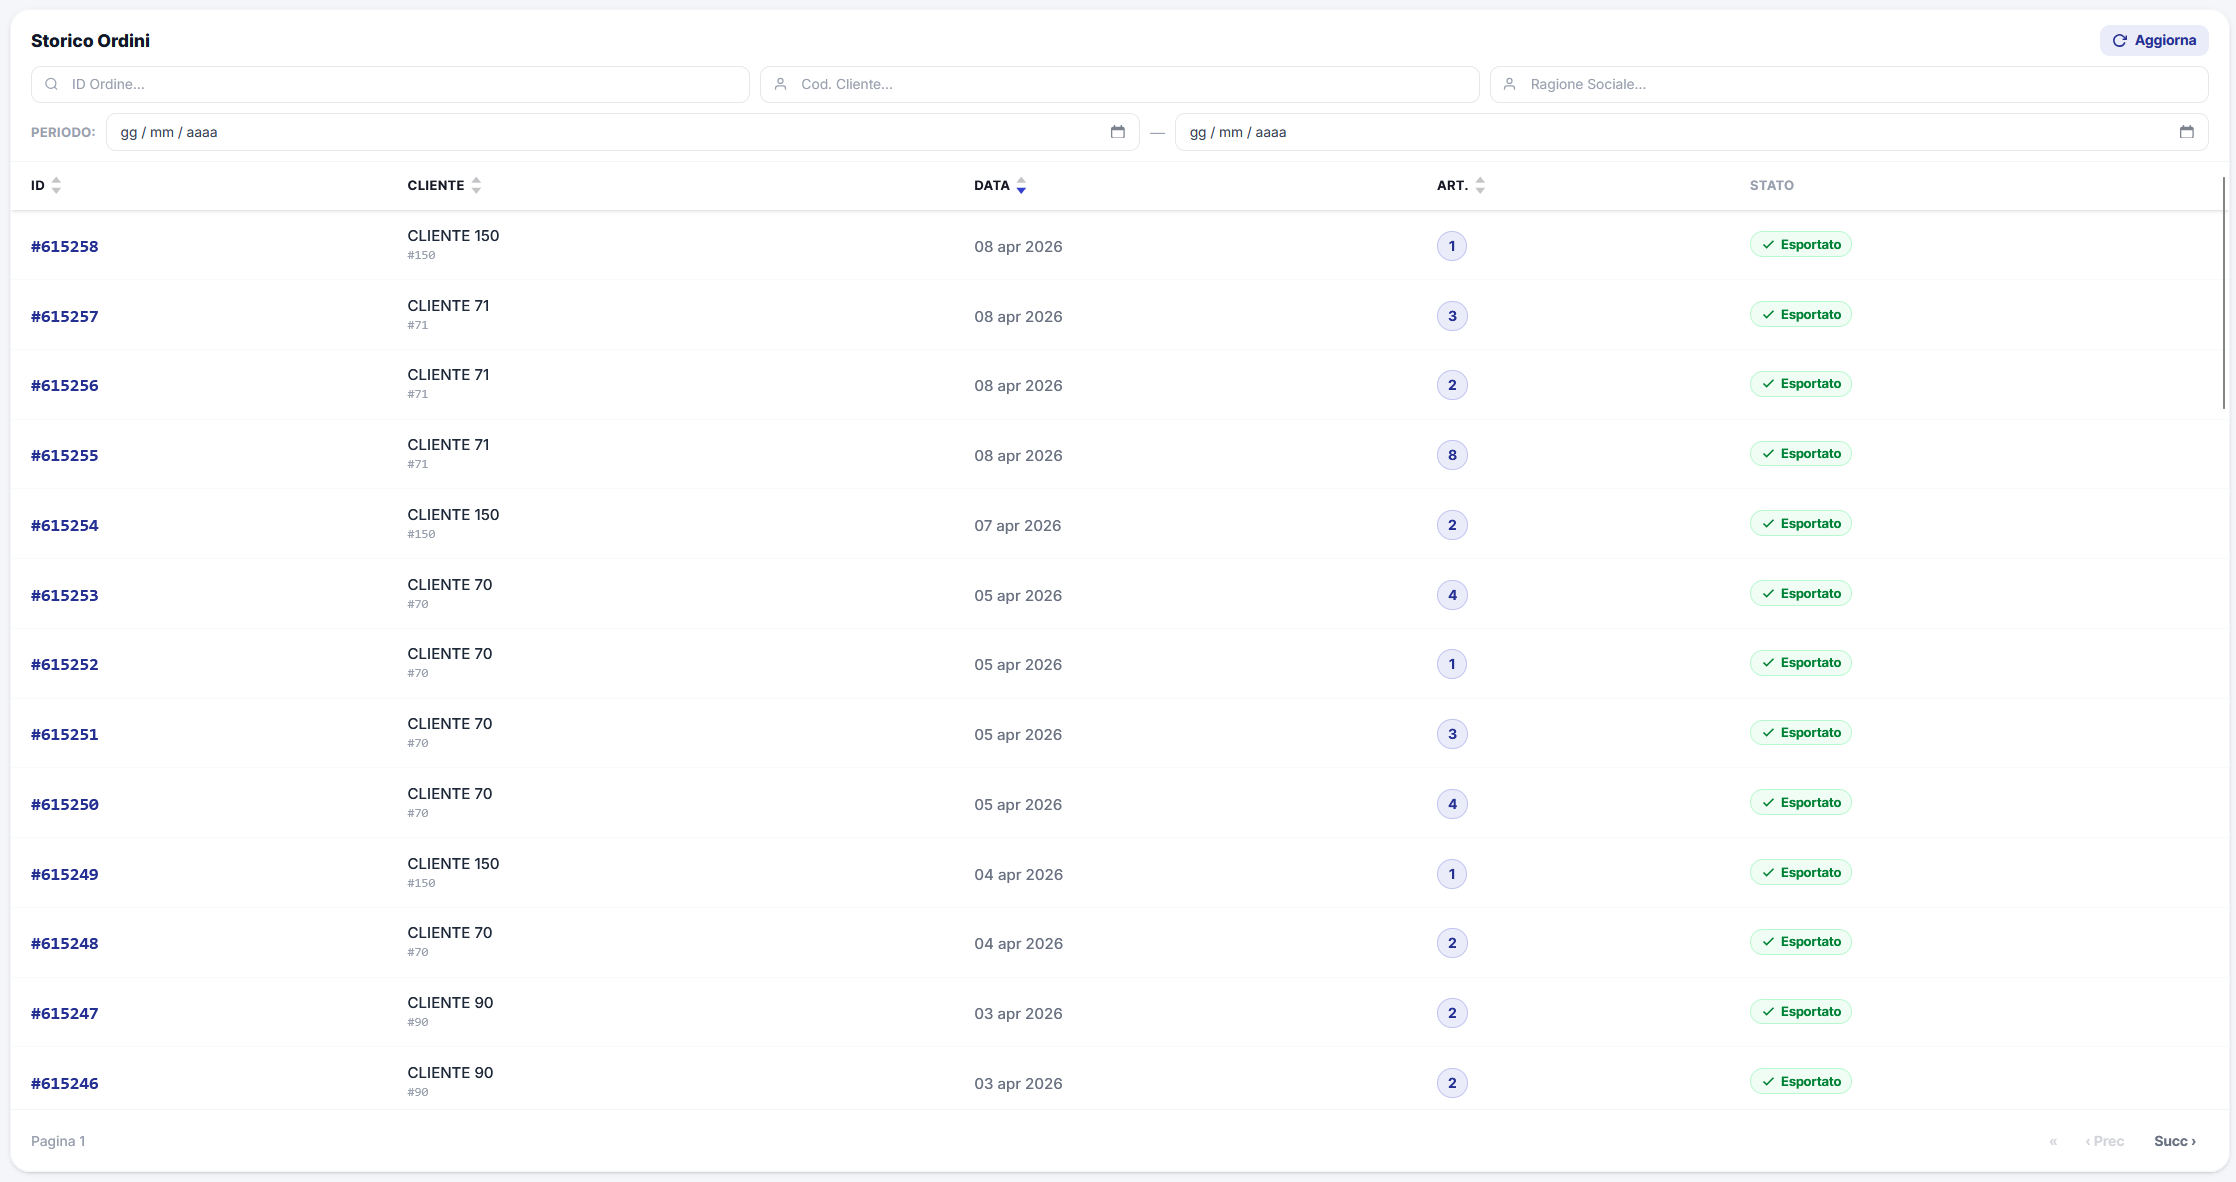
\includegraphics[width=0.7\textwidth]{Contenuti/immagini/storico operatore.png}
    \caption{Storico degli ordini}
\end{figure}

La sezione \textbf{Storico Ordini} consente la consultazione di tutti gli ordini di tutti i clienti.

\begin{enumerate}
    \item \textbf{Lista ordini}: Tabella con ordinamento multicolonna. Ogni riga mostra: ID ordine (cliccabile), ragione sociale cliente, data, numero di articoli e stato export.
    \item \textbf{Filtri avanzati}:
    \begin{itemize}
        \item Campo di ricerca per ID ordine.
        \item Campo per codice cliente.
        \item Campo per ragione sociale (ricerca debounced).
        \item Filtro per intervallo date (da -- a).
        \item Ordinamento per qualsiasi colonna (ID, cliente, data, articoli) con frecce di direzione.
    \end{itemize}
    \item \textbf{Pulsante X}: Cancella tutti i filtri attivi.
    \begin{figure}[H]
        \centering
        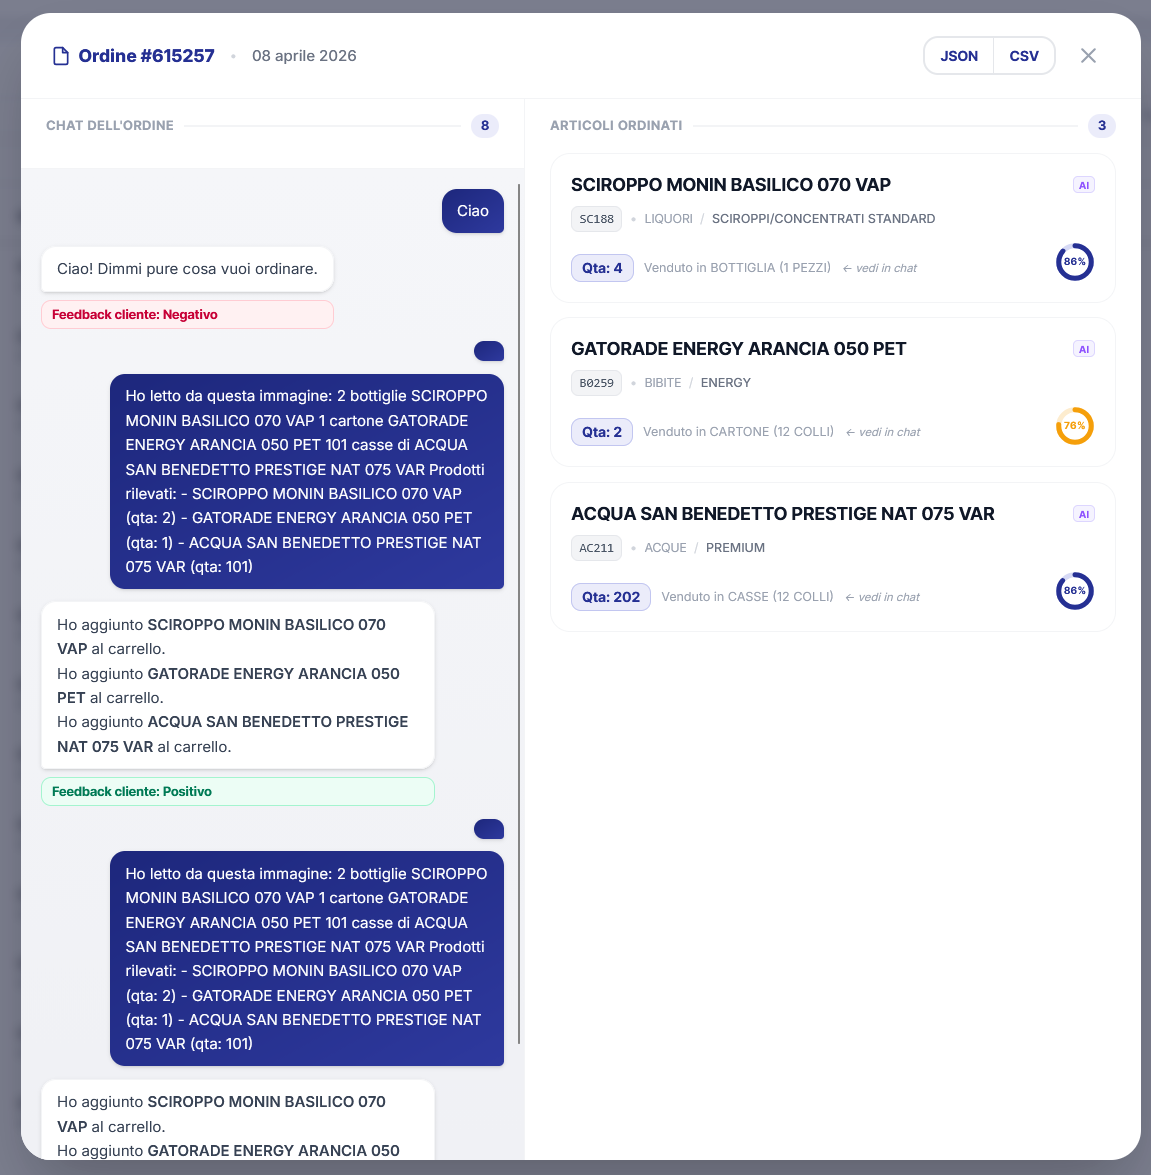
\includegraphics[width=0.7\textwidth]{Contenuti/immagini/dettagli ordine operatore.png}
        \caption{Dettagli ordine}
    \end{figure}
    \item \textbf{Dettaglio ordine}: Cliccando su una riga si apre un modale di dettaglio con:
    \begin{itemize}
        \item A sinistra: chat completa dell'ordine (se disponibile).
        \item A destra: elenco articoli ordinati con codice, descrizione, linea/famiglia, quantit\`a ordinata, unit\`a di misura e confidenza IA. Cliccando su un articolo con messaggio collegato si scrolla alla chat evidenziando il messaggio.
    \end{itemize}
    \item \textbf{Export}: Nel dettaglio ordine sono presenti i pulsanti \texttt{JSON} e \texttt{CSV} per esportare l'ordine singolarmente. Il file viene salvato nella cartella configurata nelle variabili d'ambiente.
    \item \textbf{Export batch}: Al login, se la cartella di export \`e configurata, viene eseguito automaticamente un export batch degli ordini non ancora esportati (fino a 50). Il risultato viene notificato tramite toast.
    \item \textbf{Stato export}: Nella lista ordini, la colonna \texttt{Stato} mostra un badge verde \texttt{Esportato} se l'ordine \`e gi\`a stato esportato, oppure un trattino se non ancora esportato.
\end{enumerate}

\subsection{Analytics}

\begin{figure}[H]
        \centering
        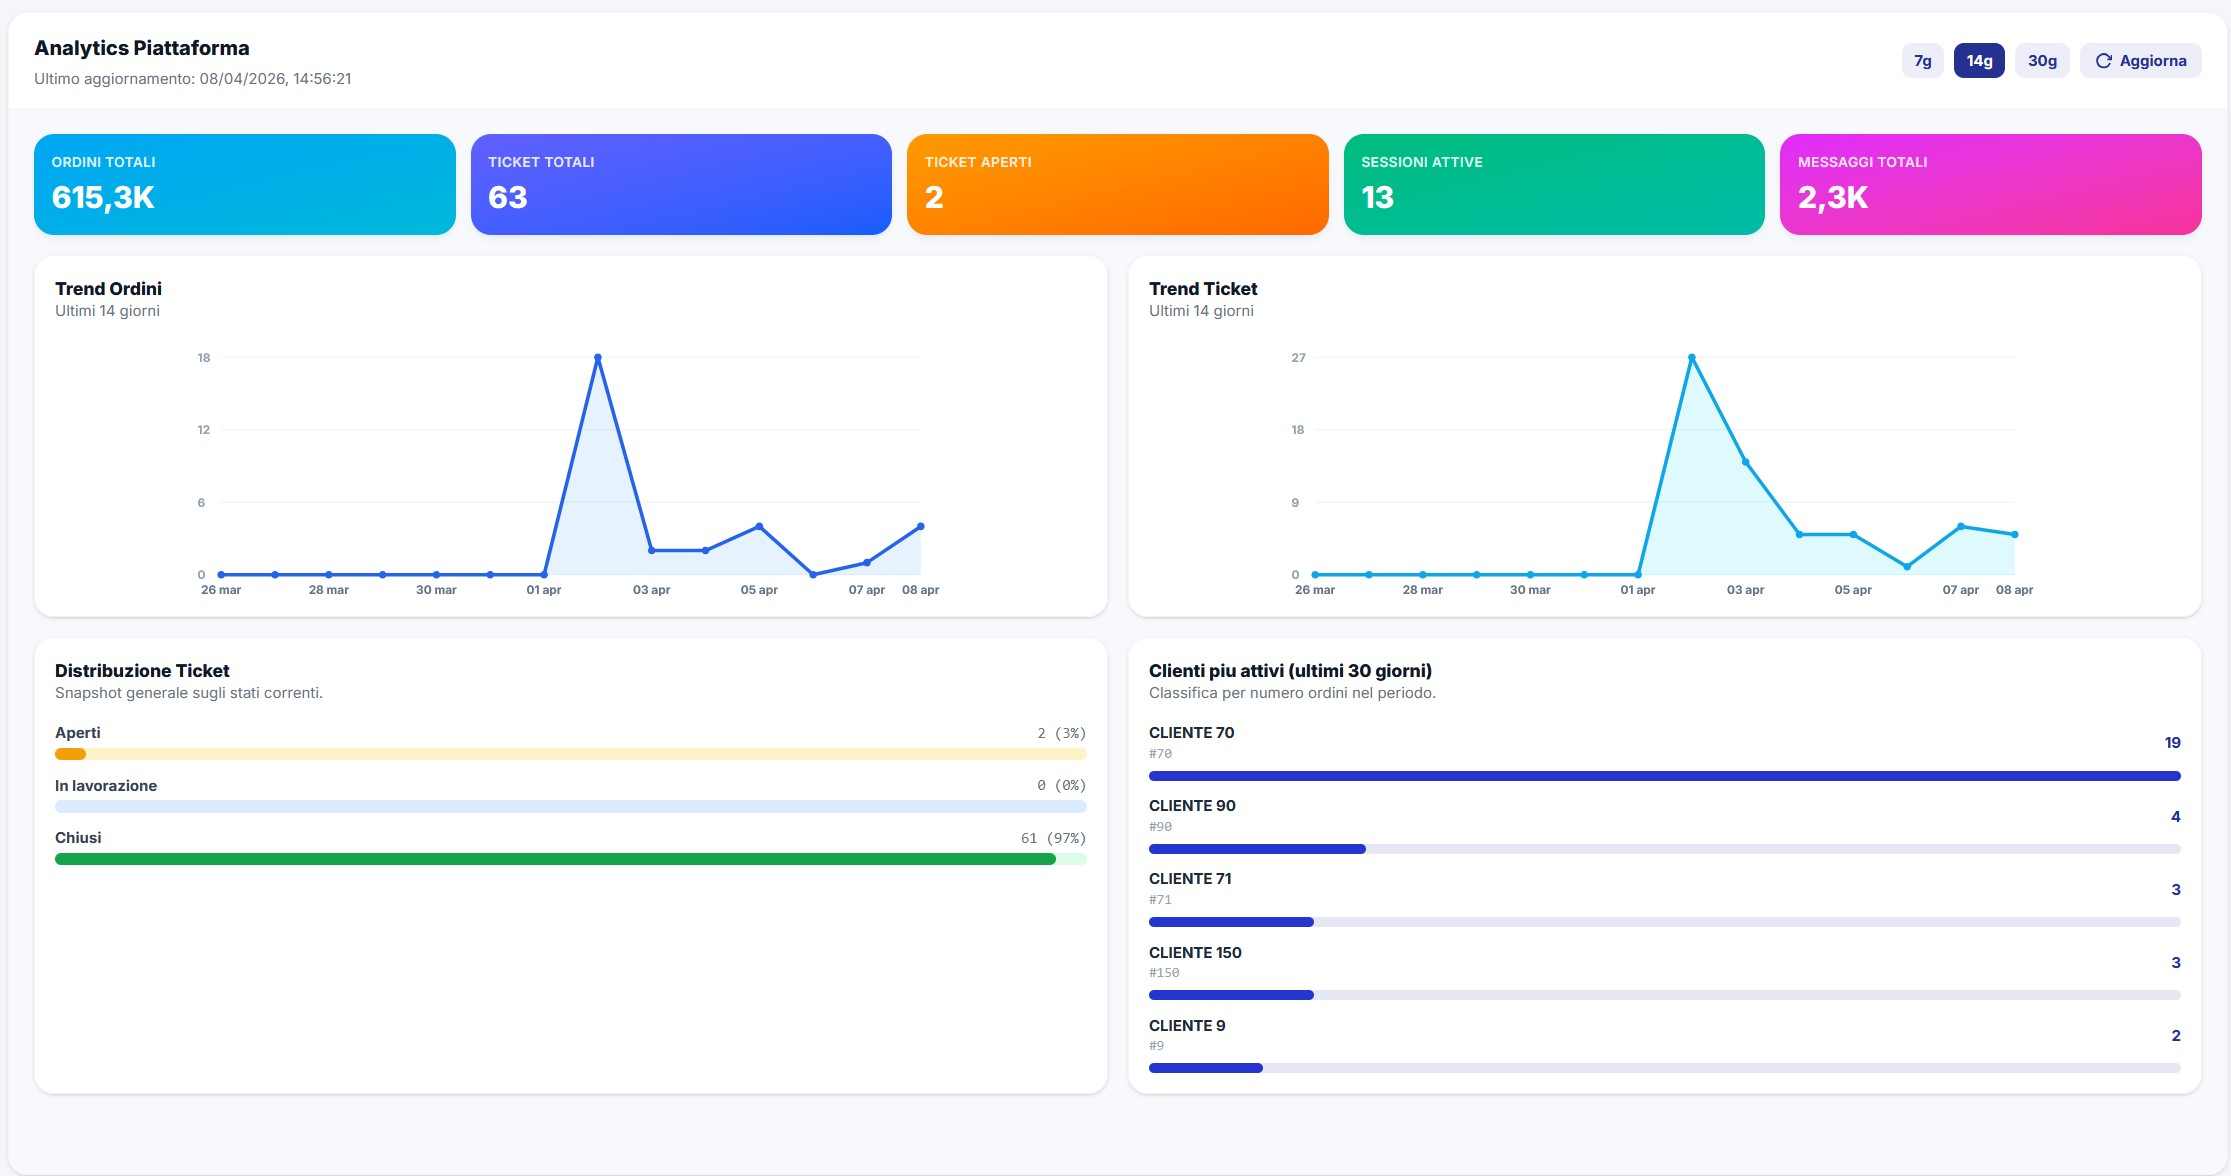
\includegraphics[width=0.8\textwidth]{Contenuti/immagini/analytics.jpeg}
        \caption{Statistiche del sistema}
    \end{figure}

È disponibile una schermata \textbf{analytics} che permette di vedere:
\begin{enumerate}
    \item Gli ordini totali effettuati dal sistema.
    \item I ticket totali.
    \item I ticket attualmente aperti
    \item Le sessioni attive al momento
    \item Il numero di messaggi inviati al sistema
    \item Il trend di ordini e tricket nel periodo scelto (7, 14 o 30 giorni)
    \item Un riepilogo dei ticket aperti, in lavorazione e chiusi
    \item L'elenco dei clienti più attivi
\end{enumerate}

\subsection{Area personale (Operatore)}

\begin{figure}[H]
    \centering
    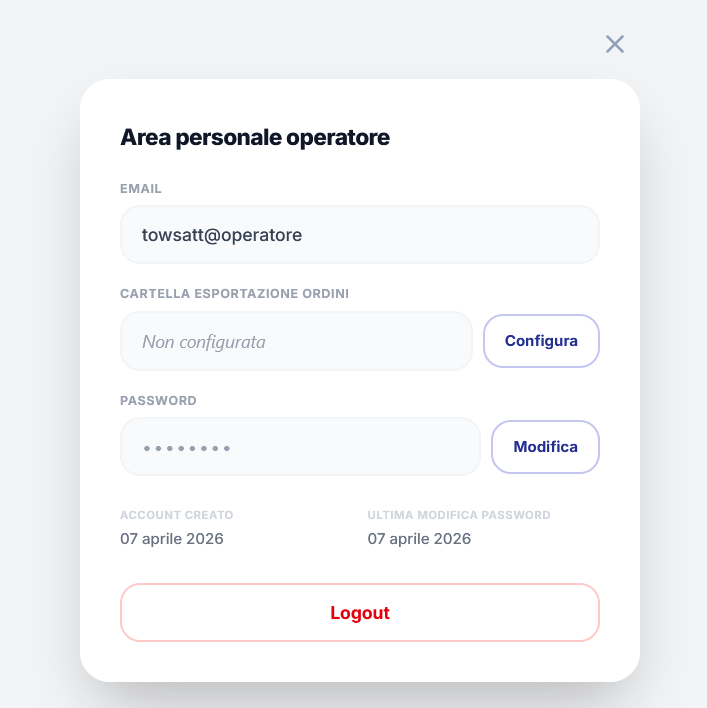
\includegraphics[width=0.7\textwidth]{Contenuti/immagini/area personale operatore.png}
    \caption{Area personale dell'operatore}
\end{figure}
\begin{figure}[H]
    \centering
    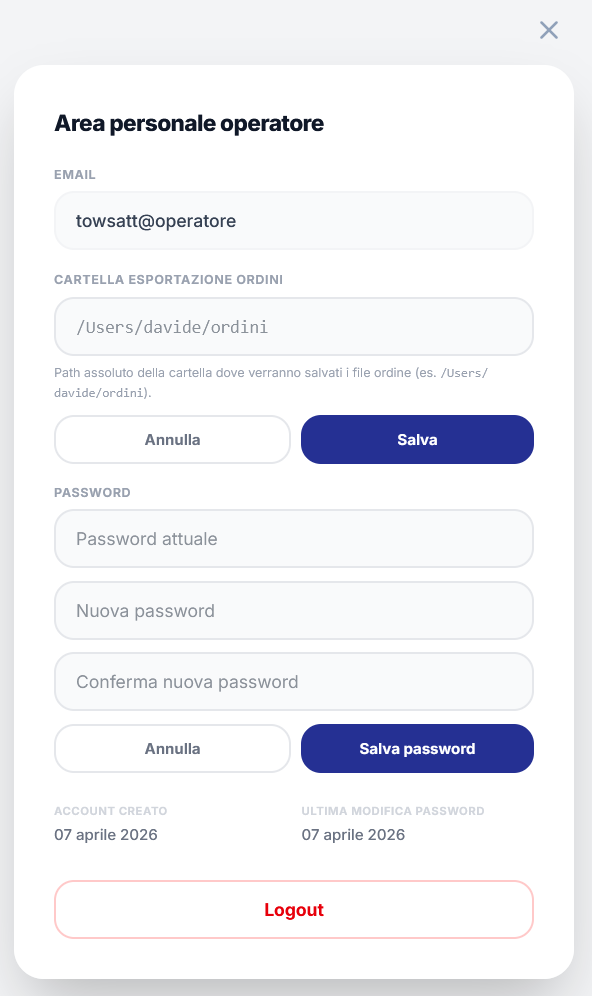
\includegraphics[width=0.7\textwidth]{Contenuti/immagini/cambio password operatore.png}
    \caption{Cambio password dell'account}
\end{figure}

Per accedere alle impostazioni del profilo:

\begin{enumerate}
    \item \textbf{Apertura}: Selezionare la sezione \texttt{Profilo} nella barra di navigazione laterale.
    \item \textbf{Dati}: Vengono mostrate email e ragione sociale dell'account operatore, oltre alle date di creazione account e ultima modifica password.
    \item \textbf{Cartella di export}: Sezione dedicata (presente solo per admin) per configurare il percorso della cartella in cui verranno salvati i file CSV/JSON degli ordini esportati. Cliccare su \texttt{Configura} o \texttt{Modifica} per impostare il path assoluto (es. \texttt{/Users/davide/ordini}), poi \texttt{Salva}.
    \item \textbf{Cambio password}: Cliccare su \texttt{Modifica} nella sezione password, inserire la password attuale, la nuova (minimo 6 caratteri) e la conferma, poi \texttt{Salva password}.
    \item \textbf{Logout}: Cliccare su \texttt{Logout} in fondo alla schermata.
\end{enumerate}
